\gls{pld} is a physical vapour deposition technique, which essentially utilizes absorption of laser energy by a target and subsequent condensation of evaporated target material on a substrate.
Like \gls{mbe} or \gls{cvd}, it is used for deposition of thin film materials.
Although not true in general \cite{lorenz2019}, a stoichiometric transfer of target composition to the substrate is attributed to \gls{pld}.
In the following, the \gls{pld} setup used for this work (Fig.~\ref{Fig:Methods_pld}a) is described.
Furthermore, an overview of the basic physical processes interplaying during a \gls{pld} process is given, based on \textcite{lorenz2019}.

\subsection{Setup}\label{Sec:Methods_pld}
The desired thin film material is provided by a ceramic pellet of the respective compound called \enquote{target}.
It is fabricated by pressing powder with high pressure into cylindrical form, before it is sintered at high temperatures.
The crystal growth takes place on a substrate, whose material is chosen to be sapphire (\ce{Al2O3}) of different crystal orientation, because it matches the symmetry of the here investigated sesquioxides.
These quadratic slabs are \qty{500}{\um} thick with an edge length of \qty{5}{\mm}.
%
In this work, oxygen is chosen as background gas to ensure fabrication of oxide thin film materials.
To control the partial pressure of the background gas, the process takes place in a vacuum chamber, called \gls{pld} chamber.
Inside the chamber, a target holder is placed opposite a sample holder, which both are capable of carrying up to four pellets and substrates, respectively.
The latter is equipped with a resistive heater, allowing growth temperatures above \qty{700}{\celsius}.
To ensure homogenous ablation and deposition, both target and substrate can be rotated, whereby a frequency of \qty{60}{\min^{-1}} is chosen in this work.
Furthermore, an offset $\varepsilon$ between the rotation centers of target and substrate is applied, i.e. the plasma plume does not hit the center of the substrate.
To achieve homogeneous thickness distributions of the deposited material, $\varepsilon=\qty{7.5}{\mm}$ is chosen.
Outside the \gls{pld} chamber, a \ce{KrF} excimer laser produces pulsed radiation, which is redirected by a mirror and enters the chamber through a fused silica window.
With a wavelength of \qty{248}{\nm}, a UV lens is needed to project the beam on the target surface, where the laser energy is absorbed.
By repositioning the lens, the laser spot size can be controlled.
The energy per pulse can be adjusted and is several hundred~\unit{\mJ} with a duration of about \qty{20}{\ns}, resulting in thousands of \unit{\kW\per\square\cm} on the target surface
    \cite{lorenz2019}.
\begin{figure}
    \centering
    \begin{tabular}{ll}
        \textbf{(a)}&\textbf{(b)}\\
        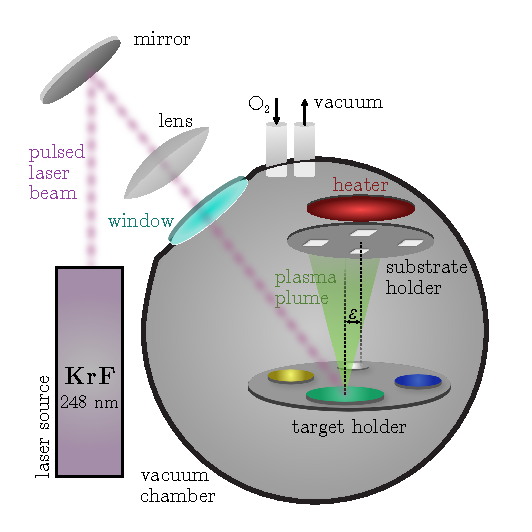
\includegraphics[width=9cm,align=c]{fastImages/PLD.pdf}&
        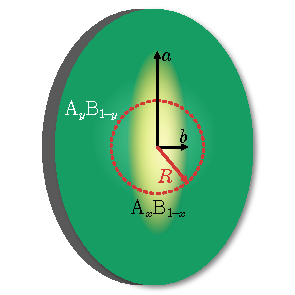
\includegraphics[width=5cm,align=c]{fastImages/target.pdf}  
    \end{tabular}
    \caption{\textbf{(a)} Schematic of a \gls{pld} setup as described in \ref{Sec:Methods_pld} \textbf{(b)} Schematic of an elliptically segmented pellet used as target for \acrshort{VCCS}-\gls{pld} (cf.~\ref{Sec:Methods_VCCS}).
    $a$ and $b$ are semi-major and semi-minor axis of the ellipse, respectively.
    $R$ denotes the radius of the circular laser spot path on the target surface.
    The composition of the inner and outer segment is \ce{A_xB_{1-x}} and \ce{A_yB_{1-y}}, respectively.}
    \label{Fig:Methods_pld}
\end{figure}

The laser energy density, called fluence $F$, can be calculated by taking the energy per pulse $E$ and the lens position $L$ into account.
For an applied $E=\qty{650}{\milli\joule}$, \qty{75}{\percent} of the energy are absorbed by mirror, lens and entrance window.
This transmittance is assumed to be independent of $E$.
The resulting fluence dependence $F(E,L)=\frac{0.25E}{A(L)}$ is visualized in Fig.~\ref{Fig:Methods_fluence}, whereby the laser spot size $A$ was measured for some $L$ and fitted by assuming parabolic behavior.

\begin{figure}
    \centering
    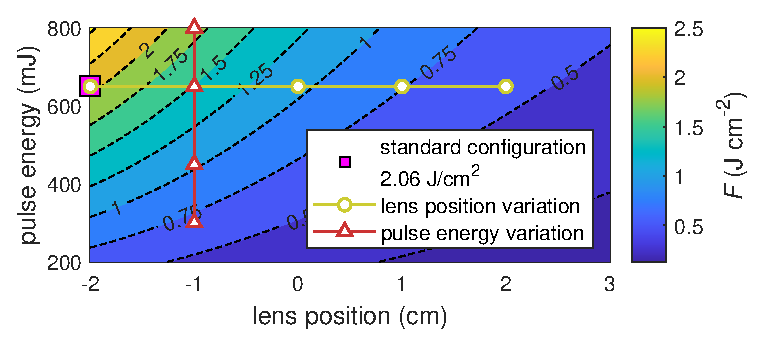
\includegraphics{fluence.eps}
    \caption{Laser energy density depending on the applied pulse energy and lens position. Smaller lens positions yield smaller spot sizes. A value of \qty{-2}{\cm} corresponds to the lens being as close as possible to the laser entrance window in the setup used for this work.
    The default configuration of \qty{650}{\milli\joule} and \qty{-2}{cm} yields typical fluences of about \qty{2}{\J\per\square\cm}.
    The triangles and circles represent the variation of laser fluence in this work, achieved by varying the pulse energy and lens position, respectively.}
    \label{Fig:Methods_fluence}
\end{figure}

\subsection{Plasma Dynamics}
The \gls{pld} procedure can be broken down into three physical processes: (i) energy absorption on the target surface, (ii) formation of a plasma and (iii) condensation on the substrate:
\begin{enumerate}[label=(\roman*)]
    \item After being projected on the surface of the pellet, the radiation penetrates the material only by a fraction of a \unit{\um}.
    Electrons are excited and oscillate in the electromagnetic field of the laser pulse, which is still ongoing.
    Those electrons collide with bulk atoms of the surface region, which are subsequently heated up and vaporize.
    This process is supported by breaking of chemical bonds due to laser radiation.
    \item A material cloud expands perpendicular to the target surface due to Coulomb repulsion and recoil.
    Absorption of remaining laser radiation results in a plasma plume which is narrow for low background partial pressures below \qty{e-4}{\milli\bar}.
    The target is rotated during this process to minimize the deflection of the plasma due to target degradation.
    The kinetic energy of the material in the plasma plume is crucial for the deposition process and can be controlled by background partial pressure and laser energy density on the target.
    \item The plasma plume hits the substrate which results in resputtering of already deposited material, which condensates together with the plasma, resulting in thermal equilibrium and thus thin film nucleation.
    A large number of adatoms results in many nucleation centers which is responsible for smooth films.
\end{enumerate}
It becomes clear, that \gls{pld} is a non-equilibrium process, making empirical optimization of growth parameters an essential part of thin film manufacturing
    \cite{lorenz2019}.

\subsection{Segmented Target Approach}\label{Sec:Methods_VCCS}
To provide a discrete material library -- a set of different samples with homogeneous composition each --, a segmented target approach as described in \textcite{vonwenckstern2020} is applied.
Specifically, the \gls{VCCS} method utilizes a segmented target, i.e.\ a target with distinct regions of different material composition.
By varying the laser spot position on the target, different plasma compositions can be achieved.
Because the target is rotating during \gls{pld}, the material distribution must be in such a way that when the radial position $R$ of the laser on the target changes, the average ablated composition $\chi(R)$ changes.
This can be realized with an elliptical segmentation, i.e.\ a target pellet with overall composition \ce{A_yB_{1-y}}, but containing an inner ellipse with composition \ce{A_xB_{1-x}} (Fig.~\ref{Fig:Methods_pld}b).
By this means, any homogeneous composition \ce{A_$\chi$B_{1-$\chi$}} with $\chi$ between $x$ and $y$ can be realized with only one target.
$\chi$ is related to the path lengths of the moving laser spot on the inner and outer segment, respectively.
The composition in the plasma can be calculated via \cite{vonwenckstern2020}:
\begin{equation}\label{Equ:Methods_composition}
    \chi(R) = y-(y-x)\frac{2}{\pi}\arccos\left[\frac{1}{\delta}\sqrt{1-\left(\frac{b}{R}\right)^2}\,\right]\,
\end{equation}
where $\delta$ and $b$ are eccentricity and semi-minor axis of the ellipse, respectively\footnote{
    The eccentricity is defined as $\delta=\sqrt{1-b^2/a^2}$, where $a$ is the length of the semi-major axis.
}.
Small and large $R$ will result in a composition equal to the composition of the inner and outer segment, respectively.
To model the process more accurately one has to take into account that the laser does not yield a point-like spot but rather an intensity distribution.
